\documentclass[a4paper,article,14pt]{extarticle}

\usepackage{spbudiploma}
\usepackage{amsmath}
\usepackage{mathtools}
\usepackage[pdftex]{graphicx}
\graphicspath{{../pictures/}}
\usepackage{listings}
\usepackage{xcolor}
\usepackage{amsfonts}
\usepackage{amsmath}
\usepackage{cases}

\usepackage{enumitem}
\definecolor{codegreen}{rgb}{0,0.6,0}
\definecolor{codegray}{rgb}{0.5,0.5,0.5}
\definecolor{codepurple}{rgb}{0.58,0,0.82}
\definecolor{backcolour}{rgb}{0.95,0.95,0.92}

\lstdefinestyle{mystyle}{
	backgroundcolor=\color{backcolour},   
	commentstyle=\color{codegreen},
	keywordstyle=\color{codegreen},
	numberstyle=\tiny\color{codegray},
	stringstyle=\color{codepurple},
	basicstyle=\ttfamily\footnotesize,
	breakatwhitespace=false,         
	breaklines=true,                 
	captionpos=b,                    
	keepspaces=false,                 
	numbers=left,                    
	numbersep=5pt,                  
	showspaces=false,                
	showstringspaces=false,
	showtabs=false,                  
	tabsize=2
}

\lstset{style=mystyle}

\begin{document}
	\begin{titlepage}
		\begin{center}
			FEDERAL STATE AUTONOMOUS EDUCATIONAL INSTITUTION
			
			OF HIGHER EDUCATION
			
			ITMO UNIVERSITY
			\vspace{3cm}
			
			\large\textbf{Report}
			
			\large on the practical task No. 8
			
			\large \flqq Practical analysis of advanced algorithms \frqq
			\vspace{5cm}
			

			\begin{flushright}
				{Performed by:} \\
				Putnikov Semyon \\ 
				J4132c \\
			\end{flushright}
			
			
			\begin{flushright}
				{Accepted by:} \\
				Dr Petr Chunaev \\ 
			\end{flushright}
			\vfill
			
			{St. Petersburg}
			\par{\number\year}
		\end{center}
	\end{titlepage}

	\newpage
	
	\section{Goal}
	Practical analysis of advanced algorithms.
	
	\section{Formulation of the problem}
	\begin{enumerate}[label=\Roman*]
		\item Choose two algorithms (interesting to you and not considered in the course) from the above-mentioned book sections.
		\item Analyse the chosen algorithms in terms of time and space complexity, design technique used, etc. Implement the algorithms and produce several experiments. Analyse the results.
	\end{enumerate}

	\section{Brief theoretical part}
	\subsection{Graham's scan}
	Graham's scan is a method of finding the convex hull of a finite set of points in the plane with time complexity O(n log n). It is named after Ronald Graham, who published the original algorithm in 1972. The algorithm finds all vertices of the convex hull ordered along its boundary. It uses a stack to detect and remove concavities in the boundary efficiently. 
	
	\subsubsection{Algorithm}
	The first step in this algorithm is to find the point with the lowest y-coordinate. If the lowest y-coordinate exists in more than one point in the set, the point with the lowest x-coordinate out of the candidates should be chosen. Call this point $P$. This step takes $O(n)$, where $n$ is the number of points in question.
	
	Next, the set of points must be sorted in increasing order of the angle they and the point $P$ make with the x-axis. Any general-purpose sorting algorithm is appropriate for this, for example heapsort (which is $O(n log n)$).
	
	Sorting in order of angle does not require computing the angle. It is possible to use any function of the angle which is monotonic in the interval $[0,\pi]$. The cosine is easily computed using the dot product, or the slope of the line may be used. If numeric precision is at stake, the comparison function used by the sorting algorithm can use the sign of the cross product to determine relative angles.
	
	The algorithm proceeds by considering each of the points in the sorted array in sequence. For each point, it is first determined whether traveling from the two points immediately preceding this point constitutes making a left turn or a right turn. If a right turn, the second-to-last point is not part of the convex hull, and lies 'inside' it. The same determination is then made for the set of the latest point and the two points that immediately precede the point found to have been inside the hull, and is repeated until a "left turn" set is encountered, at which point the algorithm moves on to the next point in the set of points in the sorted array minus any points that were found to be inside the hull; there is no need to consider these points again. (If at any stage the three points are collinear, one may opt either to discard or to report it, since in some applications it is required to find all points on the boundary of the convex hull.)
	
	Again, determining whether three points constitute a "left turn" or a "right turn" does not require computing the actual angle between the two line segments, and can actually be achieved with simple arithmetic only. For three points $P_1 = (x_1, y_1)$, $P_2 = (x_2,y_2)$ and $P_3 = (x_3, y_3)$, compute the z-coordinate of the cross product of the two vectors $\vec{P_1 P_2}$  and $\vec{P_1 P_3}$, which is given by the expression $(x_2 - x_1)(y_3 - y_1)-(y_2 - y_1)(x_3 - x_1)$. If the result is 0, the points are collinear; if it is positive, the three points constitute a "left turn" or counter-clockwise orientation, otherwise a "right turn" or clockwise orientation (for counter-clockwise numbered points).
	
	This process will eventually return to the point at which it started, at which point the algorithm is completed and the stack now contains the points on the convex hull in counterclockwise order.
	
	\subsubsection{Time complexity} 
	Sorting the points has time complexity $O(n logn)$. While it may seem that the time complexity of the loop is $O(n^2)$, because for each point it goes back to check if any of the previous points make a "right turn", it is actually O(n), because each point is considered at most twice in some sense. Each point can appear only once as a point $(x_2,y_2)$in a "left turn" (because the algorithm advances to the next point $(x_3,y_3)$ after that), and as a point $(x_2,y_2)$ in a "right turn" (because the point $(x_2,y_2)$ is removed). The overall time complexity is therefore $O(n logn)$, since the time to sort dominates the time to actually compute the convex hull. 
	
	\subsection{Gift wrapping algorithm}
	\subsubsection{Algorithm}
	For the sake of simplicity, the description below assumes that the points are in general position, i.e., no three points are collinear. The algorithm may be easily modified to deal with collinearity, including the choice whether it should report only extreme points (vertices of the convex hull) or all points that lie on the convex hull. Also, the complete implementation must deal with degenerate cases when the convex hull has only 1 or 2 vertices, as well as with the issues of limited arithmetic precision, both of computer computations and input data.
	
	The gift wrapping algorithm begins with $i=0$ and a point $p_0$ known to be on the convex hull, e.g., the leftmost point, and selects the point $p_{i+1}$ such that all points are to the right of the line $p_i p_{i+1}$. This point may be found in $O(n)$ time by comparing polar angles of all points with respect to point $p_i$ taken for the center of polar coordinates. Letting $i=i+1$, and repeating with until one reaches $p_h=p_0$ again yields the convex hull in $h$ steps. In two dimensions, the gift wrapping algorithm is similar to the process of winding a string (or wrapping paper) around the set of points.
	
	The approach can be extended to higher dimensions. 
	
	\subsubsection{Time complexity} 
	The inner loop checks every point in the set S, and the outer loop repeats for each point on the hull. Hence the total run time is $O(nh)$. The run time depends on the size of the output, so Jarvis's march is an output-sensitive algorithm.
	
	However, because the running time depends linearly on the number of hull vertices, it is only faster than $O(nlogn)$ algorithms such as Graham scan when the number $h$ of hull vertices is smaller than $logn$. Chan's algorithm, another convex hull algorithm, combines the logarithmic dependence of Graham scan with the output sensitivity of the gift wrapping algorithm, achieving an asymptotic running time $O(nlogh)$ that improves on both Graham scan and gift wrapping.

	
	\section{Results}
	%Present the results of solving the assigned problems, including graphs and tables, as well as a brief discussion of the results obtained (at most 4 pages)
	
	At Figure \ref{graham} we can se results of calculation hull by Graham's scan. Start point marked as green.
	
	\begin{figure}[h!]
		\centering
		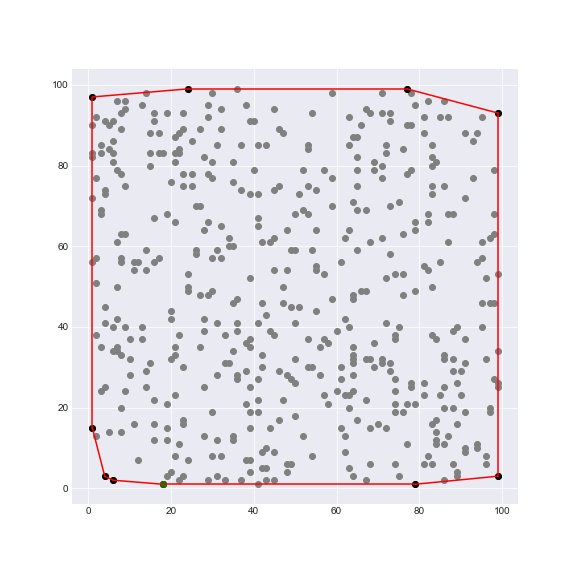
\includegraphics[scale=0.5]{graham.png}
		\caption{Results of Graham's scan.}
		\label{graham}
	\end{figure}
	
	At Figure \ref{gift} we can se results of calculation hull by Gift wrapping algorithm. Start point marked as green.

	\begin{figure}[h!]
		\centering
		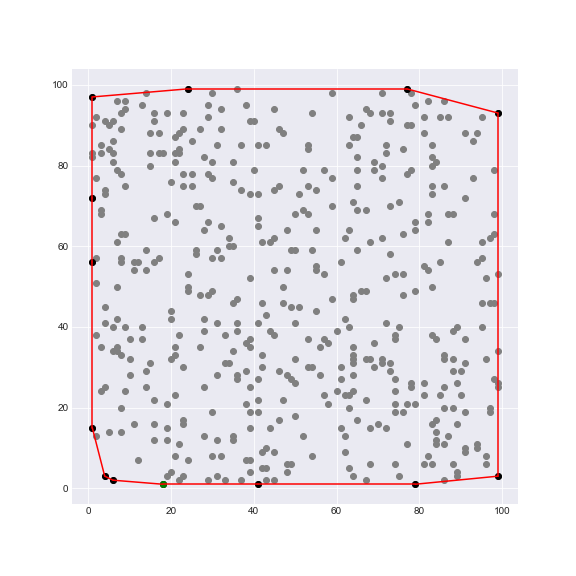
\includegraphics[scale=0.5]{gift.png}
		\caption{Result of Gift wrapping algorithm.}
		\label{gift}
	\end{figure} 
	
\end{document}